\documentclass[handout]{beamer}

\usepackage{fontspec} 
\useoutertheme{lsp}

\usepackage{lsptitle}

\def\two@digits#1{\ifnum#1<10 0\fi\number#1}
\def\mytoday{\two@digits{\number\day}.\two@digits{\number\month}.\number\year}


\usepackage{xspace,multicol}
\newcommand{\latex}{\LaTeX\xspace}
\usepackage{tikz}


\newcounter{lastpagemainpart}
\footnotesep0pt
\renewcommand{\footnoterule}{}
\usefootnotetemplate{
  \noindent
  \insertfootnotemark\insertfootnotetext}

\let\beamerfn=\footnote
\renewcommand{\footnote}[1]{%
\let\oldfnsize=\footnotesize%
\let\footnotesize=\tiny%
\beamerfn<\thebeamerpauses->{#1}%
\let\footnotesize=\oldfnsize}


\date{\mbox{24.1.2015 Open Access Netzwerk Berlin, TU Berlin}}

\usepackage{eurosym}  
 
\renewcommand{\centerline}[1]{\hfill#1\hfill\hfill\mbox{}}


\title{\mbox{Open Monograph Press}}
% \institute{FU Berlin}
\author[Nordhoff]{Sebastian Nordhoff}



\begin{document}
\lspbeamertitle

\section{Was ist OMP?}

\frame{ 
\frametitle{Was ist OMP?}
\begin{itemize}
 \item  Plattform zur Veröffentlichung von Monographien
 \item  angelehnt an OJS (Zeitschriften)
 \item  webbasiert  
 \item  Open Source
\end{itemize}
}

\frame{ 
\frametitle{Was ist OMP?}
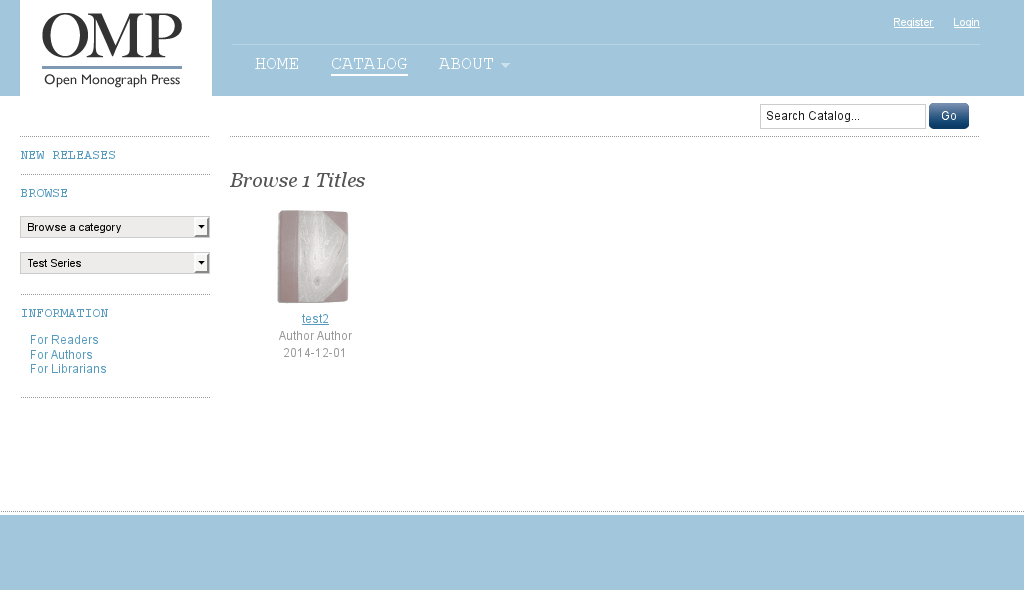
\includegraphics[width=\textwidth]{./pics/ompdev.png}
}

\frame{ 
\frametitle{Kontext}
\begin{itemize}
 \item von PKP in Kanada entwickelt
 \item weltweit eingesetzt
 \begin{itemize}
  \item in Deutschland in Heidelberg und ansatzweise in Bochum
 \end{itemize}
 \item PHP+js+CSS/LESS 
 \item kann auch für Closed Access eingesetzt werden, mit Vertriebsregionen
\end{itemize}
}



\frame{ 
\frametitle{Original}
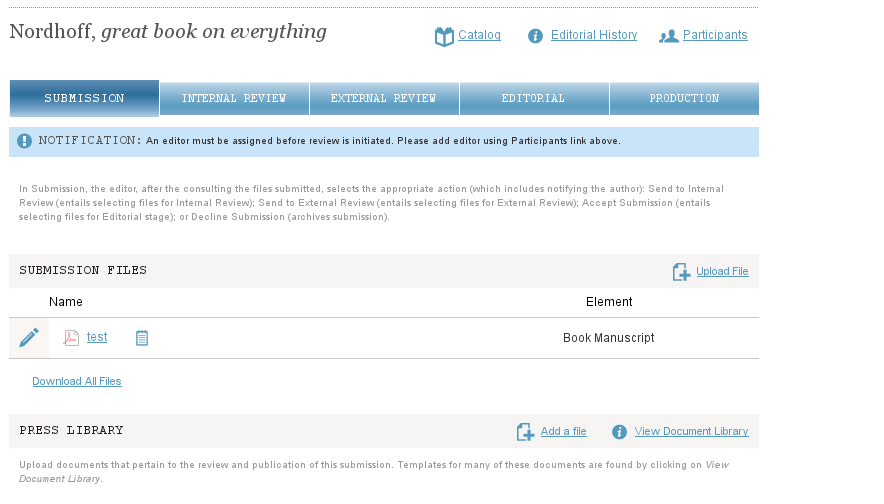
\includegraphics[width=\textwidth]{./pics/omporigsubmission.png}
}


\section{Was leistet OMP?}

\frame{ 
\frametitle{Was leistet OMP?}
\begin{itemize}
 \item   Dokumentenverwaltung
 \item   Begleitung durch den Publikationsprozess in 5 Phasen
 \item   Benutzerverwaltung mit verschiedenen Rollen
 \item   Pluginsystem
\end{itemize}
}

\frame{ 
\frametitle{OMP bei Language Science Press}
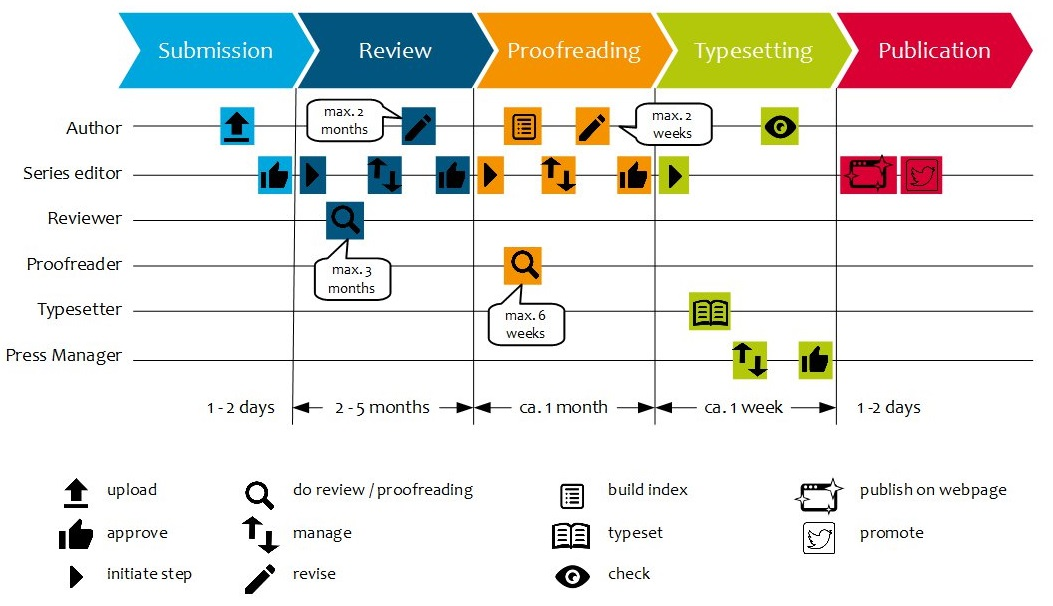
\includegraphics[width=\textwidth]{./pics/workflow.jpg}
}

\frame{ 
\frametitle{Anpassungen}
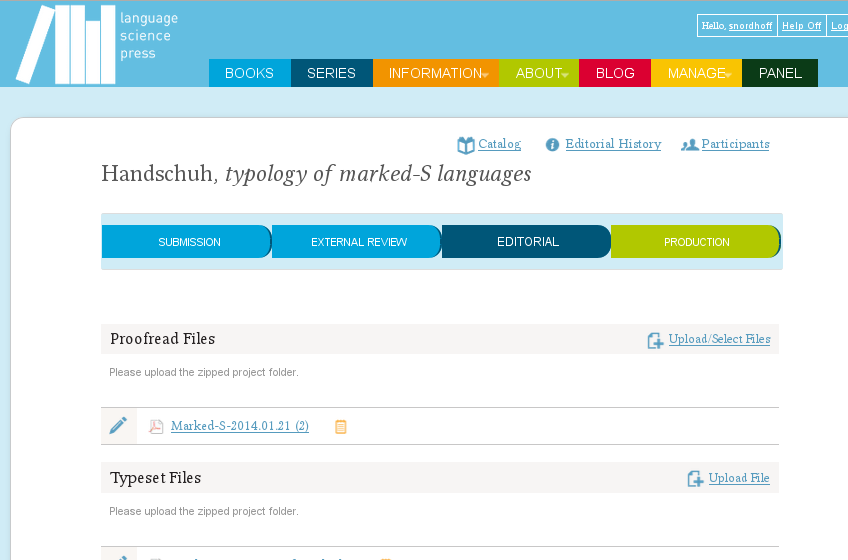
\includegraphics[width=\textwidth]{./pics/omphandschuh.png}
}



\frame{ 
\frametitle{Weitere Merkmale}
\begin{itemize}
 \item   Veröffentlichung
 \item   Metadaten
 \item   Verbreitung (OAI-PMH, Onyx, )
 \item Derzeit 19 Bücher von Language Science Press in OMP
\end{itemize}
}

\frame{ 
\frametitle{Katalogfunktion}
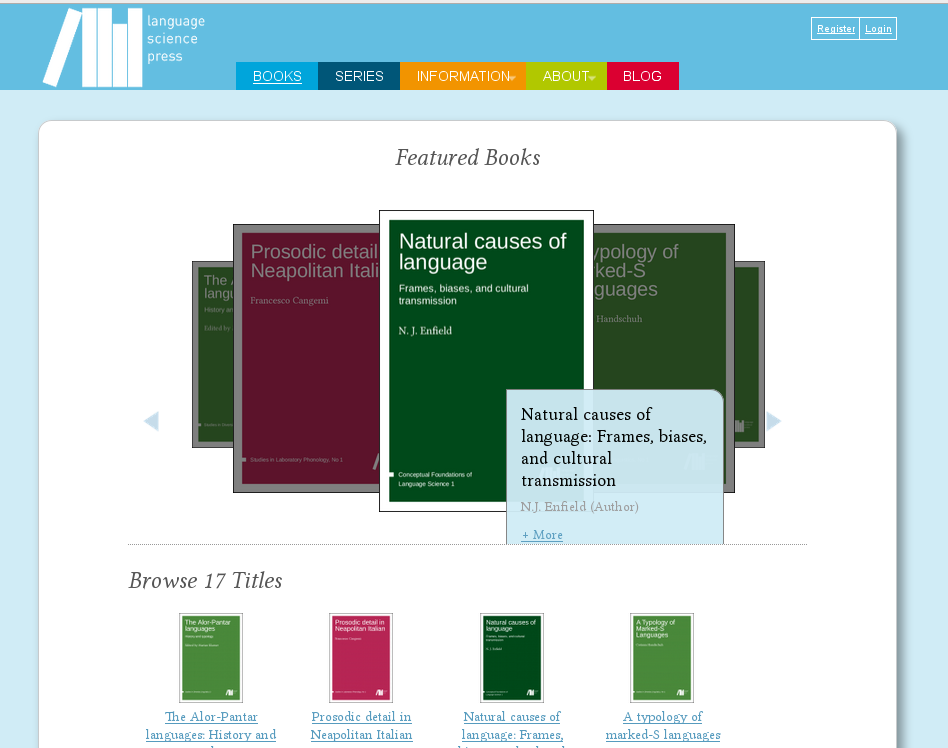
\includegraphics[width=\textwidth]{./pics/ompcatalog.png}
}

 

\section{Grenzen von OMP}
 

\frame{ 
\frametitle{Grenzen von OMP}
\begin{itemize}
 \item    von Programmierern entwickelt
 \item    Benutzerfreundlichkeit ausbaufähig
 \item    Rollensystem unklar 
 \item    Stakeholderoverkill
\end{itemize}
}


\frame{
\frametitle{Stakeholderoverkill}
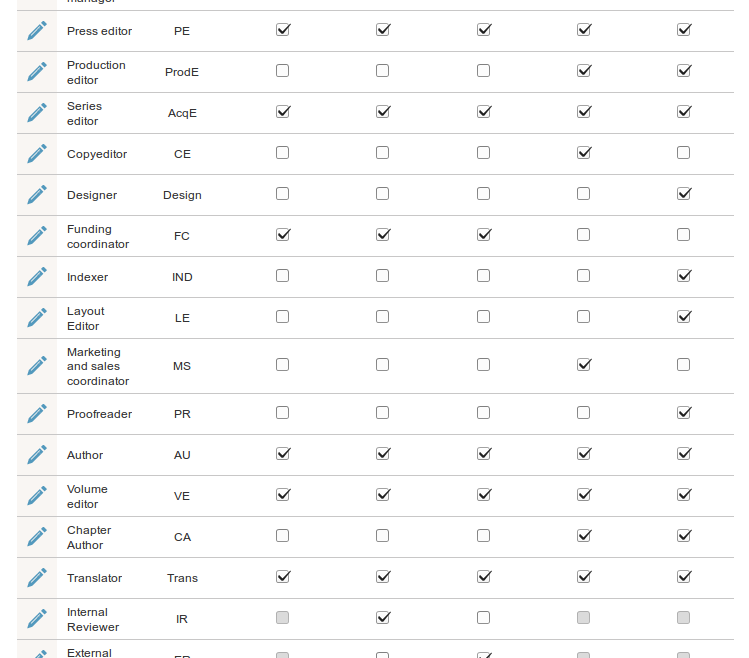
\includegraphics[width=\textwidth]{./pics/omproles.png}
}


\frame{ 
\frametitle{Grenzen von OMP}
\begin{itemize}
 \item    ISBN, DOI funktionieren noch nicht
 \item    Sammelbände (mehrere Autoren, DOIs pro Beitrag) nicht gut unterstützt
 \item derzeit bei LangSci nur von Press Managern verwendet
 \item Langsame Qualifikation der Reihenherausgeber, dann Reviewer
\end{itemize}
}



\frame{ 
\frametitle{Grenzen von OMP}
\begin{itemize}
 \item   Keine echte Versionierung der Dokumente
 \item   diverse Bugs
 \begin{itemize}
  \item fehlerhafte Benachrichtigungsfunktion
  \item Interfacefehler (Upload unmöglich, Funktionen nicht zugänglich)
 \end{itemize}
 \item   Blog extern
\end{itemize}
}

 


\section[Ausblick OMP]{Weiterentwicklung von OMP}

\frame{
\frametitle{Weiterentwicklung von OMP}
  \begin{itemize}
    \item  Höchstwahrscheinlich Orientierung an OJS 
    \item  Einbindung von Weiterentwicklungen Dritter
    \item CeDiS an der FU strebt Kompetenzausbau in diesem Bereich an
  \end{itemize}
} 
  

\frame{
\frametitle{Warum trotzdem OMP verwenden?}
  \begin{itemize}
    \item Open Source Software kann grundsätzlich verbessert werden
    \item Software noch in sehr frühem Stadium, Einflussnahmem möglich
    \item Neuentwicklung wäre technisch zwar möglich, aber Communitybuilding würde lange dauern 
  \end{itemize}
} 
  
  
\frame{ 
\frametitle{Weiterentwicklungen von LangSci}
\begin{itemize}
 \item {\bfseries LangSci Pages Plugin} 	Loads the pages needed for static pages
 \item {\bfseries Hall of Fame Plugin}	Displays Achievements of Reviewers, Typesetters, Proofreaders
 \item {\bfseries Topnavi Plugin}	Include Template for top navigation.
 \item {\bfseries Supporter Page Plugin}	Displays all supporters of Languages Science Press
 \item {\bfseries Register Plugin}		Modifies OMP-Registering
 \item {\bfseries Series Page Plugin}	Displays all series
 \item {\bfseries Simplify Workflow Plugin}	A number of smaller modifications to increase usability
 \item {\bfseries Cite-As Plugin}		Cite as.
 \item {\bfseries Remove Subtitles Plugin}	Remove subtitles in catalog view.                                
\end{itemize}
}


\frame{
\frametitle{Vielen Dank}
{\Large Fragen?} \hspace*{1em}
{\large Fragen?} \hspace*{2em}
{\huge Fragen?} \hspace*{2em}
{\large Fragen?} \hspace*{1em}
{\small Fragen?} \hspace*{2em}
{\huge Fragen?} \hspace*{2em}
{\large Fragen?} \hspace*{1em}
{\small Fragen?} \hspace*{2em}
{\scriptsize Fragen?} \hspace*{2em}
{\huge Fragen?} \hspace*{2em}
{\large Fragen?} \hspace*{1em}
{\small Fragen?} \hspace*{2em}
{\scriptsize Fragen?} \hspace*{2em}
{\Huge Fragen?} \hspace*{1em}
{\huge Fragen?} \hspace*{2em}
{\large Fragen?} \hspace*{1em}
{\small Fragen?} \hspace*{2em}
{\scriptsize Fragen?} \hspace*{2em}
{\huge Fragen?} \hspace*{2em}
{\large Fragen?} \hspace*{1em}
{\small Fragen?} \hspace*{2em}
{\scriptsize Fragen?} \hspace*{2em}
{\huge Fragen?} \hspace*{1em}
{\footnotesize Fragen?} \hspace*{1em}
{\large Fragen?} \hspace*{2em}
{\normalsize Fragen?} \hspace*{1em}
}

%\setcounter{framenumber}{\thelastpagemainpart}
\end{document}